\باب{ترچھی آمد، انعکاس، انحراف اور  انکسار}
دو خطوں کے سرحد پر عمودی آمدی موج کے انعکاس اور ترسیل پر باب \حوالہ{باب_مستوی_امواج} میں غور کیا گیا۔اس باب میں ترچھی آمدی موج کی بات کرتے ہوئے انعکاس اور ترسیل کے علاوہ انحراف اور انکسار کی بھی بات کی جائے گی۔عمودی امواج اور ترسیلی تار کے مساوات ہوبہو ایک جیسے تھے۔ ترچھی آمدی موج کی مساوی مثال ترسیلی تار میں نہیں پائی جاتی۔یہی وجہ ہے کہ ان پر یہاں علیحدہ  غور کیا جا رہا ہے۔

\حصہ{ترچھی آمد}
\جزوحصہء{عمودی قطبی برقی موج \عددیء{\kvec{E}_{\perp}}}
شکل \حوالہ{شکل_ترچھی_آمد_متوازی_برقی_میدان_عمومی_شکل} میں سرحد پر ترچھی آمد موج دکھائی گئی ہے۔سرحد \عددیء{y=0} سطح پر پایا جاتا ہے لہٰذا \عددیء{y} محدد، سرحد کے عمودی ہے۔پہلے خطے (خطہ-1) میں آمدی برقی موج \عددیء{y} محدد کے ساتھ \عددیء{\theta_i} \اصطلاح{زاویہ آمد}\فرہنگ{زاویہ!آمد}\حاشیہب{incidence angle}\فرہنگ{angle!incidence} بناتی ہے جبکہ اسی خطے میں انعکاسی برقی موج \عددیء{y} محدد کے ساتھ \عددیء{\theta_r} \اصطلاح{زاویہ انعکاس}\فرہنگ{زاویہ!انعکاس}\حاشیہب{reflection angle}\فرہنگ{angle!reflection} بناتی ہے۔ترسیلی موج دوسرے خطے (خطہ-2) میں منفی \عددیء{y} محدد کے ساتھ \عددیء{\theta_t} زاویہ بناتی ہے۔ترسیلی موج کو انحرافی موج بھی کہا جاتا ہے لہٰذا \عددیء{\theta_t} اصطلاح{زاویہ انحراف}\فرہنگ{زاویہ!انحراف}\حاشیہب{refraction angle}\فرہنگ{angle!refraction} کہلاتی ہے۔پہلے خطے کے مستقل \عددیء{\epsilon_1, \mu_1, \sigma_1, Z_1, \eta_1} جبکہ دوسرے خطے کے مستقل \عددیء{\epsilon_2, \mu_2, \sigma_2, Z_2, \eta_2} ہیں۔
\begin{figure}
\centering
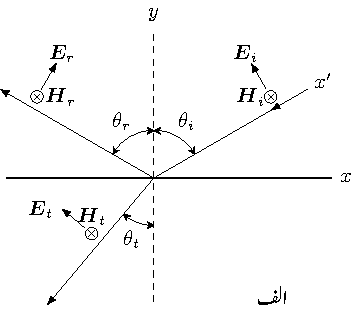
\includegraphics{figObliqueIncidenceParallelElectricField}
\caption{ترچھی آمد کی صورت میں انعکاسی اور ترسیلی امواج اور ان کے زاویے۔برقی میدان عمودی قطبیت رکھتی ہے۔}
\label{شکل_ترچھی_آمد_متوازی_برقی_میدان_عمومی_شکل}
\end{figure}

ہم دو صورتوں پر باری باری غور کریں گے۔ پہلی صورت میں برقی موج سطح آمد (یعنی $xy$ سطح) کے  عمودی ہو گی جبکہ دوسری صورت میں برقی موج اس سطح کے متوازی ہو گی۔ان دو صورتوں میں برقی موج بالترتیب \اصطلاح{عمودی قطب موج}\فرہنگ{عمودی قطب موج}\فرہنگ{قطبیت!عمودی}\حاشیہب{perpendicular polarized}\فرہنگ{polarized!perpendicular} اور \اصطلاح{متوازی قطب موج}\فرہنگ{متوازی قطب موج}\فرہنگ{قطبیت!متوازی}\حاشیہب{parallel polarized}\فرہنگ{polarized!parallel} کہلائیں گے۔شکل \حوالہ{شکل_ترچھی_آمد_متوازی_برقی_میدان_عمومی_شکل} عمودی قطبیت کی صورت حال دکھا رہی ہے۔کسی بھی عمومی برقی موج کو عمودی اور متوازی قطب کے امواج کا مجموعہ لکھا جا سکتا ہے۔

منفی \عددیء{z} سمت میں حرکت کرتی \عددیء{\ax} میدان کی برقی موج
\begin{align*}
\kvec{E}_i=E_0 \ax e^{j(\omega t +\beta_1 z)}
\end{align*} 
لکھی جاتی ہے۔اس موج میں برقی میدان ہر نقطے پر تمام اوقات \عددیء{\ax} سمت میں ہو گا جبکہ حرکت کی سمت میں فاصلہ \عددیء{z} سے ظاہر کیا جاتا ہے۔اب \عددیء{\ax} اکائی سمتیہ کی جگہ کسی بھی عمومی اکائی سمتیہ \عددیء{\kvec{a}} سمت کا میدان جو \عددیء{z} محدد کی بجائے لکیر \عددیء{l} پر گھٹتے فاصلے کی جانب حرکت کر رہا ہو
\begin{align*}
\kvec{E}_i=E_0 \kvec{a} e^{j(\omega t +\beta_1 l)}
\end{align*} 
لکھی جائے گی۔اب شکل \حوالہ{شکل_ترچھی_آمد_متوازی_برقی_میدان_عمومی_شکل} میں \عددیء{\kvec{E}_i} پر دوبارہ غور کریں۔یہ برقی میدان \عددیء{\az} سمت میں ہے جبکہ برقی موج لکیر \عددیء{x'} پر حرکت کر رہی ہے لہٰذا اس موج کو
\begin{align}\label{مساوات_ترچھا_آمد_ترچھی_کارتیسی}
\kvec{E}_i=E_0 \az e^{j(\omega t +\beta_1 x')}
\end{align}
لکھا جا سکتا ہے جہاں کارتیسی محدد \عددیء{x,y} کے مرکز سے لکیر \عددیء{x'} پر فاصلہ ناپا گیا ہے۔آئیں مساوات \حوالہ{مساوات_ترچھا_آمد_ترچھی_کارتیسی} میں لکیر \عددیء{x'} پر فاصلے کو کارتیسی محدد \عددیء{x,y} کے متغیرات استعمال کرتے ہوئے ناپیں۔
%
\begin{figure}
\centering
\begin{subfigure}{0.4\textwidth}
\centering
\includegraphics{figObliqueIncidenceParallelElectricFieldCoordinateTransformation}
\caption{فاصلے کا کارتیسی محدد میں اظہار۔}
\label{شکل_ترچھی_محدد_کی_تبدیلی}
\end{subfigure}
\begin{subfigure}{0.4\textwidth}
\centering
\includegraphics{figObliqueIncidenceParallelElectricFieldUnitVectorTransformation}
\caption{اکائی سمتیہ کا کارتیسی محدد میں اظہار۔}
\label{شکل_ترچھی_اکائی_سمتیہ}
\end{subfigure}
\caption{کسی بھی سمت میں فاصلے اور اکائی سمتیہ کو کارتیسی محدد میں لکھنے کا طریقہ۔}
\label{شکل_ترچھی_تبادلہ_فاصلہ_اور_اکائی_سمتیہ}
\end{figure}

شکل \حوالہ{شکل_ترچھی_تبادلہ_فاصلہ_اور_اکائی_سمتیہ}-الف میں آمد موج اور کارتیسی محدد دوبارہ دکھائے گئے ہیں۔اسی شکل پر ہلکی سیاہی میں لکیر \عددیء{x'} کو کارتیسی محدد \عددیء{x',y'} کا حصہ دکھایا گیا ہے۔لکیر \عددیء{x'} پر نقطہ \عددیء{A} کا مرکز سے فاصلہ \عددیء{MA} کو \عددیء{x'} لکھا گیا ہے۔ اب \عددیء{MA=MC+CA} کے برابر ہے جہاں \عددیء{{MC=x \sin \theta_i}} اور \عددیء{{CA=y \cos \theta_i}} کے برابر ہیں لہٰذا
\begin{align}
x'=x\sin \theta_i +y \cos \theta_i
\end{align} 
لکھا جا سکتا ہے جس سے ہم مساوات \حوالہ{مساوات_ترچھا_آمد_ترچھی_کارتیسی} کو
\begin{align}\label{مساوات_ترچھی_عمودی_برقی_آمدی}
\kvec{E}_i=E_0 \az e^{j[\omega t +\beta_1 (x\sin \theta_i +y \cos \theta_i)]}
\end{align}
لکھ سکتے ہیں۔

آمدی برقی اور مقناطیسی میدان \عددیء{x'} کے عمودی ہیں۔برقی میدان کی سمت \عددیء{\az} (یا $\az'$) ہے جہاں \عددیء{\az} اور \عددیء{\az'} دونوں ایک ہی سمت کو ظاہر کرتے ہیں۔مقناطیسی میدان \عددیء{\kvec{H}_i} کی سمت \عددیء{y'} محدد کی سمت میں ہے جسے \عددیء{\ay'}  لکھا جا سکتا ہے۔آئیں \عددیء{\ay'} کو کارتیسی محدد \عددیء{x,y} کے متغیرات کی صورت میں شکل \حوالہ{شکل_ترچھی_تبادلہ_فاصلہ_اور_اکائی_سمتیہ}-ب کی مدد سے لکھیں۔اکائی سمتیہ \عددیء{\ay'} کو دو سمتیوں کے مجموعے کے طور پر اس شکل میں دکھایا گیا ہے۔چونکہ اکائی سمتیہ کی لمبائی ایک کے برابر ہوتی ہے لہٰذا اس شکل میں تکون کے وتر کی لمبائی اکائی ہے۔یوں  تکون کا قاعدہ \عددیء{\cos \theta_i} اور اس کا عمود \عددیء{\sin \theta_i} کے برابر ہوں گے جس سے
\begin{align}
\ay'=-\cos \theta_i \ax+\sin \theta_i \ay
\end{align} 
لکھا جا سکتا ہے۔ان معلومات کو استعمال کرتے ہوئے آمدی مقناطیسی موج
\begin{align*}
\kvec{H}_i&=\frac{E_0}{Z_1} \ay' e^{j(\omega t +\beta_1 x')}
\end{align*}
کو
\begin{align}\label{مساوات_ترچھی_عمودی_برقی_میں_مقناطیسی_آمدی}
\kvec{H}_i=\frac{E_0}{Z_1} (-\cos \theta_i \ax+\sin \theta_i \ay) e^{j[\omega t +\beta_1 (x\sin \theta_i +y \cos \theta_i)]}
\end{align}
لکھا جا سکتا ہے۔

مساوات \حوالہ{مساوات_ترچھی_عمودی_برقی_آمدی} اور مساوات \حوالہ{مساوات_ترچھی_عمودی_برقی_میں_مقناطیسی_آمدی} کے مساوی دوری سمتی مساوات
\begin{align}
\kvec{E}_{si} & = \az E_0 e^{j\beta_1 (x\sin \theta_i +y \cos \theta_i)} \\
\kvec{H}_{si} & = (-\cos \theta_i \ax+\sin \theta_i \ay)\frac{E_0}{Z_1} e^{j\beta_1 (x\sin \theta_i +y \cos \theta_i)}
\end{align}

مساوات \حوالہ{مساوات_موج_شرح_انعکاس_تعریف} شرح انعکاس جبکہ مساوات \حوالہ{مساوات_موج_شرح_ترسیل_تعریف} شرح ترسیل کی تعریف بیان کرتے ہیں۔عین سرحد پر عمودی \عددیء{(\perp)} قطب کے میدان کے لئے ان مساوات کو
\begin{align}
\Gamma_{\perp}&=\frac{E_r}{E_i} \\
\tau_{\perp} &=\frac{E_t}{E_i}
\end{align}
لکھا جائے گا۔
\begin{figure}
\centering
\begin{subfigure}{0.4\textwidth}
\centering
\includegraphics{figObliqueIncidenceParallelElectricFieldCoordinateTransformationReflecTedWave}
\caption{انعکاسی موج کے فاصلے کارتیسی محدد میں اظہار۔}
\label{شکل_ترچھی_انعکاسی_برقی}
\end{subfigure}%
\begin{subfigure}{0.4\textwidth}
\centering
\includegraphics{figObliqueIncidenceParallelElectricFieldUnitMagneticVectorTransformation}
\caption{انعکاسی مقناطیسی موج کی اکائی سمتیہ کا کارتیسی محدد میں اظہار۔}
\label{شکل_ترچھی_انعکاسی_مقناطیسی_اکائی}
\end{subfigure}%
\caption{انعکاسی موج کے متغیرات کا کارتیسی محدد میں اظہار۔}
\label{شکل_ترچھی_اکائی_اظہار}
\end{figure}

شکل \حوالہ{شکل_ترچھی_اکائی_اظہار}-الف میں صرف انعکاسی  موج دکھائی گئی ہے۔مرکز \عددیء{M} سے موج کا فاصلہ \عددیء{l} لیتے ہوئے برقی موج کی مساوات حاصل کرتے ہیں۔تکون BAC میں \عددیء{\phase{A}=\theta_r} کے برابر ہے۔چونکہ \عددیء{{MA=MC+CA}} کے برابر ہے جہاں \عددیء{{MC=-x \sin \theta_r}} اور \عددیء{{CA=y \cos \theta_r}} کے برابر ہیں لہٰذا
\begin{align}
l=-x \sin \theta_r+y\cos \theta_r
\end{align}
لکھا جائے گا۔چونکہ نقطہ \عددیء{B} منفی محدد پر ہے لہٰذا \عددیء{MC} حاصل کرتے وقت منفی علامت کی ضرورت ہو گی۔یوں انعکاسی برقی موج
\begin{gather}
\begin{aligned}
\kvec{E}_{sr}&=\Gamma_{\perp} E_0 e^{- j \beta_1 l}\\
&=\Gamma_{\perp} E_0 e^{- j \beta_1 (-x \sin \theta_r+y\cos \theta_r)}
\end{aligned}
\end{gather}
لکھی جائے گی جہاں بڑھتے \عددیء{l} کی جانب حرکت کی بنا پر \عددیء{e} کی طاقت میں منفی کی علامت استعمال کی گئی۔

انعکاسی مقناطیسی موج کی مساوات لکھنے کی خاطر مقناطیسی میدان کی اکائی سمتیہ درکار ہے۔شکل \حوالہ{شکل_ترچھی_اکائی_اظہار}-ب میں انعکاسی مقناطیسی میدان کی سمت میں اکائی سمتیہ \عددیء{\kvec{a}_H} دکھائی گئی ہے جو \عددیء{x} محدد کے ساتھ \عددیء{\theta_r} زاویہ بناتی ہے۔اکائی سمتیہ کو محدد کے مرکز پر دوبارہ ہلکی سیاہی میں دکھایا گیا ہے جہاں اسے دو سمتیات کے مجموعے کے طور پر بھی دکھایا گیا ہے۔اس شکل سے
\begin{align}
\kvec{a}_H=\cos \theta_r \ax+\sin \theta_r \ay
\end{align}
لکھا جا سکتا ہے لہٰذا انعکاسی مقناطیسی موج
\begin{align}
\kvec{H}_{sr}=(\cos \theta_r \ax+\sin \theta_r \ay)\Gamma_{\perp} \frac{ E_0}{Z_1} e^{j \beta_1 (-x \sin \theta_r+y\cos \theta_r)}
\end{align}
لکھی جا سکتی ہے۔

یہی طریقہ کار استعمال  کرتے ہوئے ترسیلی امواج کے مساوات یوں لکھے جا سکتے ہیں
\begin{align}
\kvec{E}_{st} &=\az \tau_{\perp} E_0 e^{j \beta_2 (x \sin \theta_t+y\cos \theta_t)}\\
\kvec{H}_{st} &=(-\cos \theta_t \ax+\sin \theta_t \ay ) \tau_{\perp} \frac{E_0}{Z_2} e^{j \beta_2 (x \sin \theta_t+y\cos \theta_t)}
\end{align}
جہاں ترسیلی امواج کارتیسی محدد کے مرکز سے بڑھتے فاصلے کی طرف رواں ہیں۔یہاں غور کریں کہ دوسرے خطے میں امواج کے مساوات میں مستقل \عددیء{\beta_2} اور \عددیء{Z_2} استعمال کئے گئے ہیں۔
